\documentclass[]{article}
\usepackage{lmodern}
\usepackage{amssymb,amsmath}
\usepackage{ifxetex,ifluatex}
\usepackage{fixltx2e} % provides \textsubscript
\ifnum 0\ifxetex 1\fi\ifluatex 1\fi=0 % if pdftex
  \usepackage[T1]{fontenc}
  \usepackage[utf8]{inputenc}
\else % if luatex or xelatex
  \ifxetex
    \usepackage{mathspec}
  \else
    \usepackage{fontspec}
  \fi
  \defaultfontfeatures{Ligatures=TeX,Scale=MatchLowercase}
\fi
% use upquote if available, for straight quotes in verbatim environments
\IfFileExists{upquote.sty}{\usepackage{upquote}}{}
% use microtype if available
\IfFileExists{microtype.sty}{%
\usepackage{microtype}
\UseMicrotypeSet[protrusion]{basicmath} % disable protrusion for tt fonts
}{}
\usepackage{hyperref}
\hypersetup{unicode=true,
            pdftitle={R文本文件的语法},
            pdfauthor={黄蒙, GSCASS},
            pdfborder={0 0 0},
            breaklinks=true}
\urlstyle{same}  % don't use monospace font for urls
\usepackage{natbib}
\bibliographystyle{apalike}
\usepackage{color}
\usepackage{fancyvrb}
\newcommand{\VerbBar}{|}
\newcommand{\VERB}{\Verb[commandchars=\\\{\}]}
\DefineVerbatimEnvironment{Highlighting}{Verbatim}{commandchars=\\\{\}}
% Add ',fontsize=\small' for more characters per line
\usepackage{framed}
\definecolor{shadecolor}{RGB}{248,248,248}
\newenvironment{Shaded}{\begin{snugshade}}{\end{snugshade}}
\newcommand{\AlertTok}[1]{\textcolor[rgb]{0.94,0.16,0.16}{#1}}
\newcommand{\AnnotationTok}[1]{\textcolor[rgb]{0.56,0.35,0.01}{\textbf{\textit{#1}}}}
\newcommand{\AttributeTok}[1]{\textcolor[rgb]{0.77,0.63,0.00}{#1}}
\newcommand{\BaseNTok}[1]{\textcolor[rgb]{0.00,0.00,0.81}{#1}}
\newcommand{\BuiltInTok}[1]{#1}
\newcommand{\CharTok}[1]{\textcolor[rgb]{0.31,0.60,0.02}{#1}}
\newcommand{\CommentTok}[1]{\textcolor[rgb]{0.56,0.35,0.01}{\textit{#1}}}
\newcommand{\CommentVarTok}[1]{\textcolor[rgb]{0.56,0.35,0.01}{\textbf{\textit{#1}}}}
\newcommand{\ConstantTok}[1]{\textcolor[rgb]{0.00,0.00,0.00}{#1}}
\newcommand{\ControlFlowTok}[1]{\textcolor[rgb]{0.13,0.29,0.53}{\textbf{#1}}}
\newcommand{\DataTypeTok}[1]{\textcolor[rgb]{0.13,0.29,0.53}{#1}}
\newcommand{\DecValTok}[1]{\textcolor[rgb]{0.00,0.00,0.81}{#1}}
\newcommand{\DocumentationTok}[1]{\textcolor[rgb]{0.56,0.35,0.01}{\textbf{\textit{#1}}}}
\newcommand{\ErrorTok}[1]{\textcolor[rgb]{0.64,0.00,0.00}{\textbf{#1}}}
\newcommand{\ExtensionTok}[1]{#1}
\newcommand{\FloatTok}[1]{\textcolor[rgb]{0.00,0.00,0.81}{#1}}
\newcommand{\FunctionTok}[1]{\textcolor[rgb]{0.00,0.00,0.00}{#1}}
\newcommand{\ImportTok}[1]{#1}
\newcommand{\InformationTok}[1]{\textcolor[rgb]{0.56,0.35,0.01}{\textbf{\textit{#1}}}}
\newcommand{\KeywordTok}[1]{\textcolor[rgb]{0.13,0.29,0.53}{\textbf{#1}}}
\newcommand{\NormalTok}[1]{#1}
\newcommand{\OperatorTok}[1]{\textcolor[rgb]{0.81,0.36,0.00}{\textbf{#1}}}
\newcommand{\OtherTok}[1]{\textcolor[rgb]{0.56,0.35,0.01}{#1}}
\newcommand{\PreprocessorTok}[1]{\textcolor[rgb]{0.56,0.35,0.01}{\textit{#1}}}
\newcommand{\RegionMarkerTok}[1]{#1}
\newcommand{\SpecialCharTok}[1]{\textcolor[rgb]{0.00,0.00,0.00}{#1}}
\newcommand{\SpecialStringTok}[1]{\textcolor[rgb]{0.31,0.60,0.02}{#1}}
\newcommand{\StringTok}[1]{\textcolor[rgb]{0.31,0.60,0.02}{#1}}
\newcommand{\VariableTok}[1]{\textcolor[rgb]{0.00,0.00,0.00}{#1}}
\newcommand{\VerbatimStringTok}[1]{\textcolor[rgb]{0.31,0.60,0.02}{#1}}
\newcommand{\WarningTok}[1]{\textcolor[rgb]{0.56,0.35,0.01}{\textbf{\textit{#1}}}}
\usepackage{longtable,booktabs}
\usepackage{graphicx,grffile}
\makeatletter
\def\maxwidth{\ifdim\Gin@nat@width>\linewidth\linewidth\else\Gin@nat@width\fi}
\def\maxheight{\ifdim\Gin@nat@height>\textheight\textheight\else\Gin@nat@height\fi}
\makeatother
% Scale images if necessary, so that they will not overflow the page
% margins by default, and it is still possible to overwrite the defaults
% using explicit options in \includegraphics[width, height, ...]{}
\setkeys{Gin}{width=\maxwidth,height=\maxheight,keepaspectratio}
\usepackage[normalem]{ulem}
% avoid problems with \sout in headers with hyperref:
\pdfstringdefDisableCommands{\renewcommand{\sout}{}}
\IfFileExists{parskip.sty}{%
\usepackage{parskip}
}{% else
\setlength{\parindent}{0pt}
\setlength{\parskip}{6pt plus 2pt minus 1pt}
}
\setlength{\emergencystretch}{3em}  % prevent overfull lines
\providecommand{\tightlist}{%
  \setlength{\itemsep}{0pt}\setlength{\parskip}{0pt}}
\setcounter{secnumdepth}{5}
% Redefines (sub)paragraphs to behave more like sections
\ifx\paragraph\undefined\else
\let\oldparagraph\paragraph
\renewcommand{\paragraph}[1]{\oldparagraph{#1}\mbox{}}
\fi
\ifx\subparagraph\undefined\else
\let\oldsubparagraph\subparagraph
\renewcommand{\subparagraph}[1]{\oldsubparagraph{#1}\mbox{}}
\fi

%%% Use protect on footnotes to avoid problems with footnotes in titles
\let\rmarkdownfootnote\footnote%
\def\footnote{\protect\rmarkdownfootnote}

%%% Change title format to be more compact
\usepackage{titling}

% Create subtitle command for use in maketitle
\providecommand{\subtitle}[1]{
  \posttitle{
    \begin{center}\large#1\end{center}
    }
}

\setlength{\droptitle}{-2em}

  \title{R文本文件的语法}
    \pretitle{\vspace{\droptitle}\centering\huge}
  \posttitle{\par}
  \subtitle{Use R!}
  \author{黄蒙, GSCASS}
    \preauthor{\centering\large\emph}
  \postauthor{\par}
      \predate{\centering\large\emph}
  \postdate{\par}
    \date{2019-09-21}

\usepackage{ctex}

%\usepackage{xltxtra} % XeLaTeX的一些额外符号
% 设置中文字体
\setCJKmainfont[BoldFont={黑体},ItalicFont={楷体}]{新宋体}

\usepackage{amsthm,mathrsfs}
\usepackage{booktabs}
\usepackage{longtable}
\makeatletter
\def\thm@space@setup{%
  \thm@preskip=8pt plus 2pt minus 4pt
  \thm@postskip=\thm@preskip
}
\makeatother

\begin{document}
\maketitle
\begin{abstract}
随着近年来R语言相关环境的功能越来越丰富,编写包含R代码的文本文件,再通过统一的R环境运算、编译和导出,成为了一种管理文件的新方法。这种方法的好处有:(1)节省了硬盘资源,使多种多样的文件都能以文本的方式保存;(2)使针对原始数据所做的一切整理和分析工作变得可复制,实践了``可重复性研究''的理念;(3)能让作者专注于文件内容和参数调整本身,而把调节格式、修改结果的工作全部交给R并实现自动化。本文通过对markdown、Rmarkdown和bookdown的语法的整理,便利了R文本文件的编写。
\end{abstract}

{
\setcounter{tocdepth}{2}
\tableofcontents
}
\hypertarget{section}{%
\section*{首要参考文献}\label{section}}
\addcontentsline{toc}{section}{首要参考文献}

\href{https://bookdown.org/yihui/rmarkdown/}{\emph{R Markdown: The Definitive Guide}}

\hypertarget{html-}{%
\section{html 语法}\label{html-}}

html 语法大都可以在Rmarkdown中使用

\hypertarget{section-1}{%
\subsection{文字颜色}\label{section-1}}

代码:\texttt{\textless{}font\ color=\textquotesingle{}blue\textquotesingle{}\textgreater{}\ 蓝色文字。\ \textless{}/font\textgreater{}}

效果: 蓝色文字。

\hypertarget{section-2}{%
\subsection{字号}\label{section-2}}

代码:\texttt{\textless{}font\ size\ =\ 4\textgreater{}\ 4号字。\textless{}/font\textgreater{}\ \textless{}font\ size\ =\ 6\textgreater{}\ 6号字。\textless{}/font\textgreater{}}

效果: 4 号字。 6 号字。

\hypertarget{section-3}{%
\subsection{图片}\label{section-3}}

代码:\texttt{\textless{}center\textgreater{}\textless{}img\ src="地址"\ width\ =\ "50\%"\ height\ =\ \textquotesingle{}100\textquotesingle{}...\ /\textgreater{}\textless{}center/\textgreater{}}

代码:\texttt{\textless{}div\ align\ =\ center\textgreater{}\ \textless{}img\ src="地址"\ ...\ /\textgreater{}\ \textless{}/div\textgreater{}}

效果:

\hypertarget{markdown}{%
\section{markdown基本语法}\label{markdown}}

\hypertarget{section-4}{%
\subsection{段内换行}\label{section-4}}

行末\texttt{\textless{}br/\textgreater{}}或两个以上空格 + 回车为段内换行,连续两个回车为新起一段

我是第一段第一行\\
我是第一段第二行

我是第二段,注意正常的行间距和段间距

\hypertarget{section-5}{%
\subsection{增加段间距}\label{section-5}}

用\texttt{\textless{}br/\textgreater{}},每多一个就多一次换行;或\texttt{\&nbsp;},表示一个空段落。

正常段间距

正常段间距
连续两次换行,虽然看上去行距很大,但仍在一段中

~

中间隔了一个空段落,空段落可以叠加

\hypertarget{section-6}{%
\subsection{注释}\label{section-6}}

用\texttt{\textless{}!-\/-\ \ -\/-\textgreater{}}括住的内容会被注释掉,不显示在最终输出中。

\hypertarget{section-7}{%
\subsection{引用}\label{section-7}}

在引用中可以使用其他 Markdown 语法

\hypertarget{section-8}{%
\subsubsection{单层和嵌套引用}\label{section-8}}

\begin{quote}
张三说:李四这样说过
\end{quote}

\begin{quote}
\begin{quote}
不想当将军的木匠不是好厨子。
\end{quote}
\end{quote}

\hypertarget{section-9}{%
\subsubsection{多行引用}\label{section-9}}

仍然是一段(推荐):

\begin{quote}
第一行\\
第二行
\end{quote}

\begin{quote}
第一行

第二行
\end{quote}

变成了两段(不推荐):

\begin{quote}
第一段
\end{quote}

\begin{quote}
第二段
\end{quote}

\hypertarget{section-10}{%
\subsection{分隔线}\label{section-10}}

三个以上的\texttt{*/-/\_}

\begin{center}\rule{0.5\linewidth}{\linethickness}\end{center}

\hypertarget{section-11}{%
\subsection{链接}\label{section-11}}

\hypertarget{section-12}{%
\subsubsection{直接表示:}\label{section-12}}

格式为\texttt{\textless{}地址\textgreater{}}或\texttt{地址}(仅限 http 和 www 开头,这是 GFM 扩展语法)。如:百度的网址是 \url{http://www.baidu.com} 或 www.baidu.com,我的邮箱是 \href{mailto:humoonruc@126.com}{\nolinkurl{humoonruc@126.com}}。

\hypertarget{section-13}{%
\subsubsection{行内链接}\label{section-13}}

格式为\texttt{{[}链接名{]}(地址)}。如:点击超链接\href{http://www.baidu.com}{百度}

\hypertarget{section-14}{%
\subsubsection{引用式链接}\label{section-14}}

当链接被重复使用时,最好使用引用链接形式。可以将链接标记理解为一个地址变量。

在某处(比如文章结尾)定义一些链接标识符,语法为:\texttt{{[}链接标识符{]}:网址}。定义语句不会显示在输出中。正文中使用时,语法为:\texttt{{[}链接名{]}{[}链接标识符{]}},如:

在\href{https://www.google.com.hk}{Google 首页}查询 IT 资料通常是第一步,虽然在中文搜索方面\href{https://www.google.com.hk}{这个国际巨头}的用户体验常常不如\href{https://www.baidu.com}{百度}。

\hypertarget{section-15}{%
\subsection{图片}\label{section-15}}

\begin{enumerate}
\def\labelenumi{\arabic{enumi}.}
\item
  行内图片:\\
  \texttt{!{[}图片名称{]}("图片地址或网址")}
  不建议使用这种方法,编译pdf有时会报错。
\item
  引用式图片:与链接类似,也可以在文章某处定义图片的标识符,然后把行内图片引用中图片地址替换成图片标识符即可。
\end{enumerate}

\hypertarget{section-16}{%
\subsection{列表}\label{section-16}}

\hypertarget{section-17}{%
\subsubsection{列表嵌套}\label{section-17}}

用\texttt{Tab}缩进表示下一级

\begin{itemize}
\tightlist
\item
  第一级

  \begin{itemize}
  \tightlist
  \item
    第二级

    \begin{itemize}
    \tightlist
    \item
      第三级
    \item
      第三级
    \end{itemize}
  \item
    第二级
  \end{itemize}
\end{itemize}

\hypertarget{section-18}{%
\subsubsection{列表缩进}\label{section-18}}

若列表项无换行,一个空格即可;若列表项有换行,建议无序列表用三个空格如\texttt{-\ \ \ xxx},有序列表用两个空格如\texttt{1.\ \ xxx}

\begin{itemize}
\tightlist
\item
  这个列表项\\
  有换行
\item
  这个没有
\end{itemize}

\begin{enumerate}
\def\labelenumi{\arabic{enumi}.}
\tightlist
\item
  这个有序列表项\\
  有换行
\item
  这个没有
\end{enumerate}

\hypertarget{section-19}{%
\subsubsection{列表项间空行}\label{section-19}}

无换行的列表项之间不建议空行;有换行的列表项之间建议空一行;列表开始和末尾都空一行

无换行:

\begin{itemize}
\tightlist
\item
  抽烟
\item
  喝酒
\item
  烫头
\end{itemize}

有换行:

\begin{itemize}
\item
  抽很多的\\
  烟
\item
  喝酒
\item
  烫头
\end{itemize}

\hypertarget{section-20}{%
\subsection{任务列表}\label{section-20}}

\textbf{2019年读书计划}

\begin{itemize}
\tightlist
\item[$\boxtimes$]
  《R in Action》
\item[$\boxtimes$]
  《R for Data Science》
\item[$\square$]
  《Python 疯狂讲义》
\end{itemize}

\hypertarget{section-21}{%
\subsection{管道表}\label{section-21}}

\begin{longtable}[]{@{}lcr@{}}
\caption{\label{tab:easytable} 管道表}\tabularnewline
\toprule
Tables & Are & Cool\tabularnewline
\midrule
\endfirsthead
\toprule
Tables & Are & Cool\tabularnewline
\midrule
\endhead
col 3 is & right-aligned & \$1600\tabularnewline
col 2 is & centered & \$12\tabularnewline
zebra stripes & are neat & \$1\tabularnewline
\bottomrule
\end{longtable}

注:

\begin{enumerate}
\def\labelenumi{\arabic{enumi}.}
\tightlist
\item
  英文冒号 : 使列获得了某种对齐方式。
\item
  代码块和引用块不能插入表格。
\item
  管道表不允许输入单元格换行,单元格内容太宽时转换结果可能自动换行。
\item
  \texttt{Table:\ (\textbackslash{}\#tab:label)\ text},为markdown简易表自动加表编号和表名(text),写在简易表的前后均可。
\end{enumerate}

\hypertarget{Rmarkdown}{%
\section{R Markdown语法}\label{Rmarkdown}}

\hypertarget{section-22}{%
\subsection{基本语法}\label{section-22}}

\begin{itemize}
\tightlist
\item
  删除线 \texttt{a\textasciitilde{}\textasciitilde{}b\textasciitilde{}\textasciitilde{}} 他是个\sout{天才}疯子。
\item
  上标 \texttt{text\^{}supscript\^{}} a\textsuperscript{2}
\item
  下标 \texttt{text\textasciitilde{}subscript\textasciitilde{}} k\textsubscript{1}
\item
  添加脚注 \texttt{text\^{}{[}footnote{]}} 某观点\footnote{文献题录。}
\end{itemize}

\begin{verbatim}
代码块设置,使块中文字右对齐,仅适用于 pdf
\end{verbatim}

\hypertarget{r}{%
\subsection{R代码块}\label{r}}

行内代码如:2019-09-21

\begin{Shaded}
\begin{Highlighting}[]
\KeywordTok{def}\NormalTok{ print_name():}
    \BuiltInTok{print}\NormalTok{(}\StringTok{"Markdown"}\NormalTok{)}
\end{Highlighting}
\end{Shaded}

代码块

\begin{Shaded}
\begin{Highlighting}[]
\KeywordTok{sin}\NormalTok{(pi}\OperatorTok{/}\DecValTok{2}\NormalTok{)}
\end{Highlighting}
\end{Shaded}

\begin{verbatim}
[1] 1
\end{verbatim}

\hypertarget{r-1}{%
\subsection{R表格}\label{r-1}}

表格尽量使用代码块,便于统一编号

\begin{Shaded}
\begin{Highlighting}[]
\NormalTok{table <-}\StringTok{ }\NormalTok{tibble}\OperatorTok{::}\KeywordTok{tibble}\NormalTok{(}\DataTypeTok{ID =} \DecValTok{1}\OperatorTok{:}\DecValTok{5}\NormalTok{, }\DataTypeTok{name =}\NormalTok{ letters[}\DecValTok{1}\OperatorTok{:}\DecValTok{5}\NormalTok{])}
\NormalTok{knitr}\OperatorTok{::}\KeywordTok{kable}\NormalTok{(table, }\DataTypeTok{caption =} \StringTok{'order of letters'}\NormalTok{)}
\end{Highlighting}
\end{Shaded}

\begin{table}

\caption{\label{tab:unnamed-chunk-4}order of letters}
\centering
\begin{tabular}[t]{r|l}
\hline
ID & name\\
\hline
1 & a\\
\hline
2 & b\\
\hline
3 & c\\
\hline
4 & d\\
\hline
5 & e\\
\hline
\end{tabular}
\end{table}

\hypertarget{r-2}{%
\subsection{R图}\label{r-2}}

插图全部使用代码块,便于统一编号

\begin{Shaded}
\begin{Highlighting}[]
\CommentTok{# knitr::include_graphics("figs/myfig01.png")}
\end{Highlighting}
\end{Shaded}

\hypertarget{section-23}{%
\subsection{公式}\label{section-23}}

\begin{itemize}
\tightlist
\item
  行内公式:将公式包在\texttt{\$\ \$}之间,如:\(\sin\pi/2=\) 1\\
\item
  独立公式:将公式包含在\texttt{\$\$\ \$\$}之间,如:
\end{itemize}

\[
  f(x)=\frac{1}{2} \sum_{j=1}^{\infty} \int_{0}^{1} \sin ^{2}(j t x) d t
\]

\begin{itemize}
\tightlist
\item
  为了产生对齐的公式,在独立公式中使用aligned环境。公式中的环境以\texttt{\textbackslash{}begin\{环境名\}}开始,以\texttt{\textbackslash{}end\{环境名\}}结束,用\texttt{\textbackslash{}\textbackslash{}}表示换行,用\texttt{\&}表示一个上下对齐位置。如:
\end{itemize}

\[
\begin{aligned}
  f(x) =& \sum_{k=0}^\infty \frac{1}{k!} x^k \\
  =& e^x
\end{aligned}
\]

\begin{itemize}
\tightlist
\item
  为公式手动编号
  \[
  y = f(x) \tag{label}
  \]
\end{itemize}

显然,手动编号不是一个好主意。

\hypertarget{section-24}{%
\subsection{制表式截面}\label{section-24}}

仅适用于html格式

\hypertarget{by-product}{%
\subsubsection{By Product}\label{by-product}}

(tab content)

\hypertarget{by-region}{%
\subsubsection{By Region}\label{by-region}}

(tab content)

\hypertarget{bookdown}{%
\section{bookdown语法}\label{bookdown}}

bookdown比Rmarkdown的主要升级之处在于自动编号和交叉引用。

\hypertarget{section-25}{%
\subsection{章节编号和引用}\label{section-25}}

\hypertarget{section-26}{%
\subsubsection{编号}\label{section-26}}

\texttt{\#\ (PART)\ 第一篇\ \{-\}} 部分(篇)
\texttt{\#\ References\ \{-\}} 参考文献
\texttt{\#\ (APPENDIX)\ 附录\ \{-\}} 附录

\hypertarget{section-27}{%
\subsubsection{引用}\label{section-27}}

\begin{enumerate}
\def\labelenumi{\arabic{enumi}.}
\tightlist
\item
  \texttt{\{\#tag\}},自动为标题编号,并定义标题的标签,便于引用。标签只能含字母、数字和连字符``-'',图、表标签同
\item
  \texttt{\{-\}},不为标题编号,也不定义标签
\item
  \texttt{\{\#tag\ .unnumbered\}},设置标题的标签,但不为标题编号
\item
  \texttt{\textbackslash{}@ref(tag)},引用标题编号。如第\ref{bookdown}节是关于bookdown的。
\end{enumerate}

\hypertarget{usage-writing-fig}{%
\subsection{图形自动编号}\label{usage-writing-fig}}

用R代码块生成的图形,只要具有代码块标签label,且提供代码段选项\texttt{fig.cap="图题"},就可对图形自动编号,并且可以用如\texttt{\textbackslash{}@ref(fig:label)}的格式引用图形。如:

\begin{Shaded}
\begin{Highlighting}[]
\KeywordTok{plot}\NormalTok{(}\DecValTok{1}\OperatorTok{:}\DecValTok{10}\NormalTok{)}
\end{Highlighting}
\end{Shaded}

\begin{figure}

{\centering 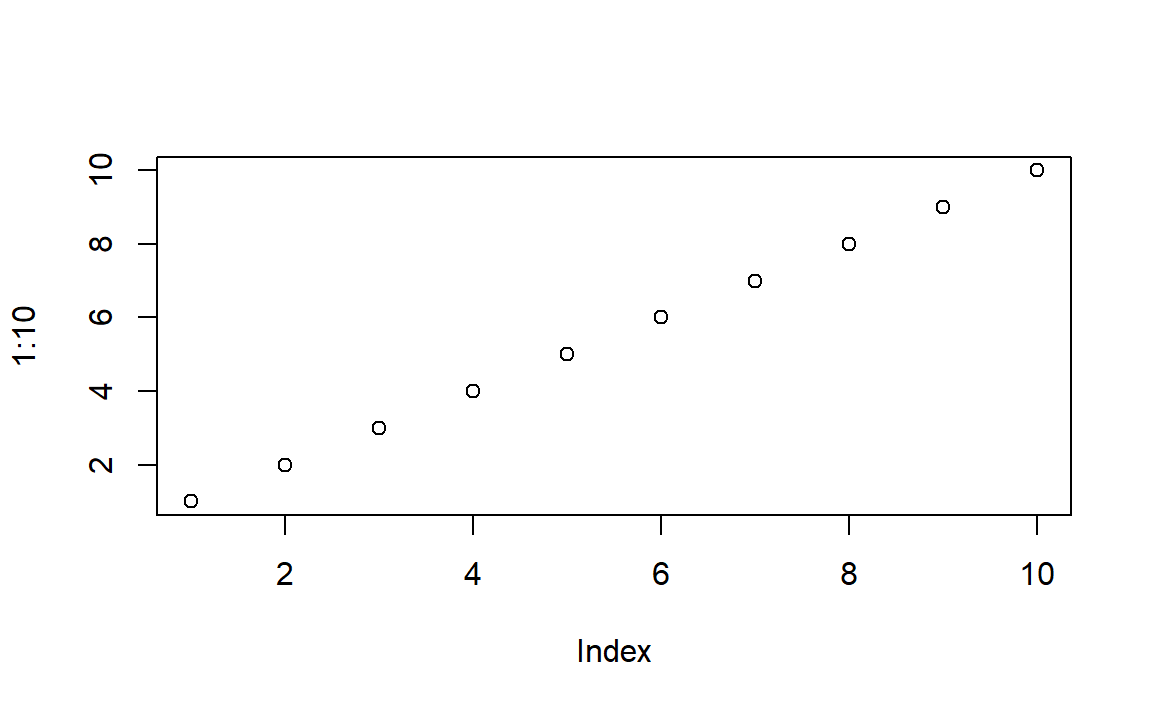
\includegraphics[width=0.8\linewidth]{Figs/u-w-f-ex01-1} 

}

\caption{测试图}\label{fig:u-w-f-ex01}
\end{figure}

引用如:参见图\ref{fig:u-w-f-ex01},其中的\texttt{fig:}是必须的。

\hypertarget{usage-writing-tab}{%
\subsection{表格自动编号}\label{usage-writing-tab}}

用R代码\texttt{knitr::kable()}生成的表格,只要具有代码块标签,并且在\texttt{knitr::kable()}调用时加选项\texttt{caption="表题"},就可以对表格自动编号,并且可以用如\texttt{\textbackslash{}@ref(tab:label)}的格式引用表格。如:

\begin{Shaded}
\begin{Highlighting}[]
\NormalTok{d <-}\StringTok{ }\KeywordTok{data.frame}\NormalTok{(}\StringTok{"自变量"}\NormalTok{ =}\StringTok{ }\DecValTok{1}\OperatorTok{:}\DecValTok{10}\NormalTok{, }\StringTok{"因变量"}\NormalTok{ =}\StringTok{ }\NormalTok{(}\DecValTok{1}\OperatorTok{:}\DecValTok{10}\NormalTok{)}\OperatorTok{^}\DecValTok{2}\NormalTok{)}
\NormalTok{knitr}\OperatorTok{::}\KeywordTok{kable}\NormalTok{(d, }\DataTypeTok{caption =} \StringTok{"1到10的平方"}\NormalTok{, }\DataTypeTok{longtable =} \OtherTok{TRUE}\NormalTok{ )}
\end{Highlighting}
\end{Shaded}

\begin{longtable}{r|r}
\caption{\label{tab:u-w-tab-ex01}1到10的平方}\\
\hline
自变量 & 因变量\\
\hline
1 & 1\\
\hline
2 & 4\\
\hline
3 & 9\\
\hline
4 & 16\\
\hline
5 & 25\\
\hline
6 & 36\\
\hline
7 & 49\\
\hline
8 & 64\\
\hline
9 & 81\\
\hline
10 & 100\\
\hline
\end{longtable}

引用如:参见表\ref{tab:u-w-tab-ex01},其中的\texttt{tab:}是必须的。

\hypertarget{usage-writing-math}{%
\subsection{数学公式编号}\label{usage-writing-math}}

不需要编号的公式,仍可以按照一般的Rmd文件使用行内的\texttt{\$\ \$}或独立的\texttt{\$\$\ \$\$}公式块。

需要编号的公式,写在\texttt{\textbackslash{}begin\{align\}}和\texttt{\textbackslash{}end\{align\}}之间。然后,对不需要编号的\textbf{行}在末尾用\texttt{\textbackslash{}nonumber}标注;对需要编号的\textbf{行}用\texttt{(\textbackslash{}\#eq:mylabel)}添加自定义标签,在正文的引用中使用与上面相同的格式\texttt{\textbackslash{}@ref(eq:mylable)}。如:

\begin{align}
f(x) =& \sum_{k=0}^\infty \frac{1}{k!} x^k \label{eq:efunc-sum} \\
  = e^x \label{eq:efunc-ex}
\end{align}

\begin{align}
\Sigma =&  (\sigma_{ij})_{n\times n} \nonumber \\
=& E[(\boldsymbol{X} - \boldsymbol{\mu}) (\boldsymbol{X} - \boldsymbol{\mu})^T ] \label{eq:var-mat-def}
\end{align}

引用如:协方差定义见式\eqref{eq:var-mat-def}。

\hypertarget{section-28}{%
\subsection{文献引用与文献列表}\label{section-28}}

\begin{enumerate}
\def\labelenumi{\arabic{enumi}.}
\tightlist
\item
  将所有文献用bib格式保存为一个\texttt{.bib}文献库,如模板中的样例文件\texttt{mybib.bib}。用\texttt{@item}和\texttt{{[}@item{]}}引用文献题录,如\footnote{没有方括号时,题录前后一定要加空格。}:
\end{enumerate}

\begin{longtable}[]{@{}ll@{}}
\toprule
\begin{minipage}[b]{0.47\columnwidth}\raggedright
源代码\strut
\end{minipage} & \begin{minipage}[b]{0.47\columnwidth}\raggedright
效果\strut
\end{minipage}\tabularnewline
\midrule
\endhead
\begin{minipage}[t]{0.47\columnwidth}\raggedright
\texttt{@MWP06-HighStat}\strut
\end{minipage} & \begin{minipage}[t]{0.47\columnwidth}\raggedright
\citet{MWP06-HighStat}\strut
\end{minipage}\tabularnewline
\begin{minipage}[t]{0.47\columnwidth}\raggedright
\texttt{@Lin2018\ {[}page.\ 33{]}}\strut
\end{minipage} & \begin{minipage}[t]{0.47\columnwidth}\raggedright
\citet[page. 33]{Lin2018}\strut
\end{minipage}\tabularnewline
\begin{minipage}[t]{0.47\columnwidth}\raggedright
\texttt{{[}@Lin2018,\ page.\ 33{]}}\strut
\end{minipage} & \begin{minipage}[t]{0.47\columnwidth}\raggedright
\citep[page. 33]{Lin2018}\strut
\end{minipage}\tabularnewline
\begin{minipage}[t]{0.47\columnwidth}\raggedright
\texttt{{[}@Lin2018;\ @MWP06-HighStat{]}}\strut
\end{minipage} & \begin{minipage}[t]{0.47\columnwidth}\raggedright
\citep{Lin2018, MWP06-HighStat}\strut
\end{minipage}\tabularnewline
\begin{minipage}[t]{0.47\columnwidth}\raggedright
\texttt{{[}see\ @Lin2018,\ page.\ 33-35;\ also\ @MWP06-HighStat,\ ch.\ 1{]}}\strut
\end{minipage} & \begin{minipage}[t]{0.47\columnwidth}\raggedright
\citetext{\citealp[see][page. 33-35]{Lin2018}; \citealp[also][ch.~1]{MWP06-HighStat}}\strut
\end{minipage}\tabularnewline
\begin{minipage}[t]{0.47\columnwidth}\raggedright
\texttt{{[}-@Lin2018{]}}\strut
\end{minipage} & \begin{minipage}[t]{0.47\columnwidth}\raggedright
\citeyearpar{Lin2018}\strut
\end{minipage}\tabularnewline
\bottomrule
\end{longtable}

\begin{enumerate}
\def\labelenumi{\arabic{enumi}.}
\setcounter{enumi}{1}
\tightlist
\item
  将
\end{enumerate}

\begin{verbatim}
nocite:|
@item1,@item2
\end{verbatim}

写在YAML文件头中,表示某些文献不直接引用,只在末尾参考文献列表中出现。

被引用的文献将出现在一章末尾以及全书的末尾,对PDF输出则仅出现在全书末尾。

\hypertarget{section-29}{%
\subsection{索引}\label{section-29}}

\texttt{\textbackslash{}index\{索引词汇\}},标记为索引,仅适用于pdf格式,输出在文末。

\hypertarget{section-30}{%
\subsection{编译}\label{section-30}}

\texttt{bookdown::render\_book(\textquotesingle{}index.Rmd\textquotesingle{},\ \textquotesingle{}bookdown::epub\_book\textquotesingle{})}

\texttt{bookdown::render\_book(\textquotesingle{}index.Rmd\textquotesingle{},\ \textquotesingle{}bookdown::pdf\_book\textquotesingle{})}

\texttt{bookdown::render\_book(\textquotesingle{}index.Rmd\textquotesingle{},\ \textquotesingle{}bookdown::gitbook\textquotesingle{})}

只编译一章:\\
\texttt{bookdown::render\_book(\textquotesingle{}chapter1.rmd\textquotesingle{},\ \textquotesingle{}bookdown::gitbook\textquotesingle{},\ preview\ =\ T)}

\bibliography{mybib.bib}


\end{document}
